\section{Data and Summary Statistics}
\label{s:data}

To investigate the effects of the construction of Brasília's subway system on its citizens income, we use geographic and socioeconomic data from the Brazilian Institute of Geography and Statistics (IBGE). Specifically, we use census-tract data for Brasília from the 2000 and 2010 censuses.\footnote{Brazil's census happens once every ten years. The 1980 and 1991 censuses are not used because neither provides micro-geographic data disaggregated at the census-tract level, making pre-trend analysis at this level of spatial resolution infeasible.} Our main outcome is tract-level per capita income and its change over 2000--2010. Per capita income is constructed, for each census tract and year, as the ratio of the sum of nominal monthly income declared by household heads to the total number of residents in permanent private dwellings.\footnote{The numerator captures only the income declared by the household head, not the total income of all residents. This restriction is data-driven: the 2000 Census does not publish total income of all persons in the universe of census tracts, providing only income distributions by bracket. Two features support the validity of this measure for the purposes of this study. First, since the numerator is defined identically in both years, any systematic underestimation cancels in the 2000--2010 log difference, preserving the interpretation of the coefficient as relative income growth. Second, household heads are more likely than other household members to be long-term, stable residents of the same census tract across both census years. Changes in the head's income between 2000 and 2010 therefore more plausibly reflect genuine earnings improvements for incumbent residents---those who were already living in the tract before and after subway access---rather than compositional change driven by new, higher-income arrivals. This aligns directly with the real income gains interpretation pursued in this study. Any additional income gains accruing to other household members are not captured, so the estimates constitute a lower bound on the total household income effect of subway access.} We also use baseline (2000) tract characteristics as controls: distance to Brasília's CBD, population, the share with completed higher education, the illiteracy rate, and the share of residents aged 65+. The reason why we focus on these two years is because Brasília's subway system began operating in 2001, meaning we have data from before and after the subway's implementation. Data for the subway lines and stations, as well as the geographic boundaries the Administrative Regions,\footnote{The Federal District (DF) has no municipalities; it is divided into Administrative Regions (Regiões Administrativas, RAs), subdistrict units used for local public administration and statistical reporting.} were obtained from the Brasília GeoPortal (GeoPortal/DF), which provides cartographic and urban-planning information for the capital. For the instrumentation of Brasília's subway system we use the abandoned (planned but not built) project sketch produced by the Mauá Institute of Technology.

The 2000 and 2010 Censuses use different census-tract boundaries: in 2010, many 2000 tracts were split (subdivided), meaning the original polygon was divided into two or more smaller polygons. To make the statistical analyses in this study feasible, we harmonize the 2010 census-tract map with the 2000 census-tract map; the formal details of this procedure are described in Appendix~\ref{s:appendix_harmonization}.

Our analysis focuses on census tracts located within a 10 km radius of the nearest subway station. This restriction is motivated by comparability: tracts far from the subway network are likely to differ systematically from those plausibly affected by the subway system in terms of urban form, land-use regulation, baseline socioeconomic conditions, and broader patterns of development. By limiting the sample to a relatively narrow band around the subway network, we compare ``treated'' tracts (those closer to stations) to ``control'' tracts that are geographically proximate and embedded in the same metropolitan context, reducing concerns that estimated differences in income dynamics are driven by large-scale spatial heterogeneity rather than by subway access. To define exposure, we classify a tract as treated if it lies within 1 km of the nearest subway station. This choice follows the Institute for Transportation and Development Policy (ITDP) \emph{People Near Transit} metric, which adopts a 1 km radius to capture the maximum distance most users are willing to walk to access metro service \citep{marks2016people}. This threshold corresponds roughly to a 10--15 minute walk and is widely used in the empirical literature as a reasonable catchment area for mass transit stations \citep{iamtrakul2024exploring, yang2024does, mohammad2017effect}. Given this localized nature of accessibility gains, restricting the estimation sample to tracts within 10 km of a station helps ensure that the control group consists of locations for which the subway is at most a marginal amenity, strengthening the credibility of the counterfactual. Figure~\ref{fig:1} reports the spatial distribution of census tracts and subway infrastructure in Brasília for 2000 and 2010 with harmonized census tracts.

\begin{figure}[h!]
\caption{Spatial Distribution of Census Tracts and Subway Infrastructure in Brasília}
\label{fig2a}
\vspace{-0.4cm}
    \centering
    \begin{subfigure}[b]{0.49\textwidth}
        \centering
        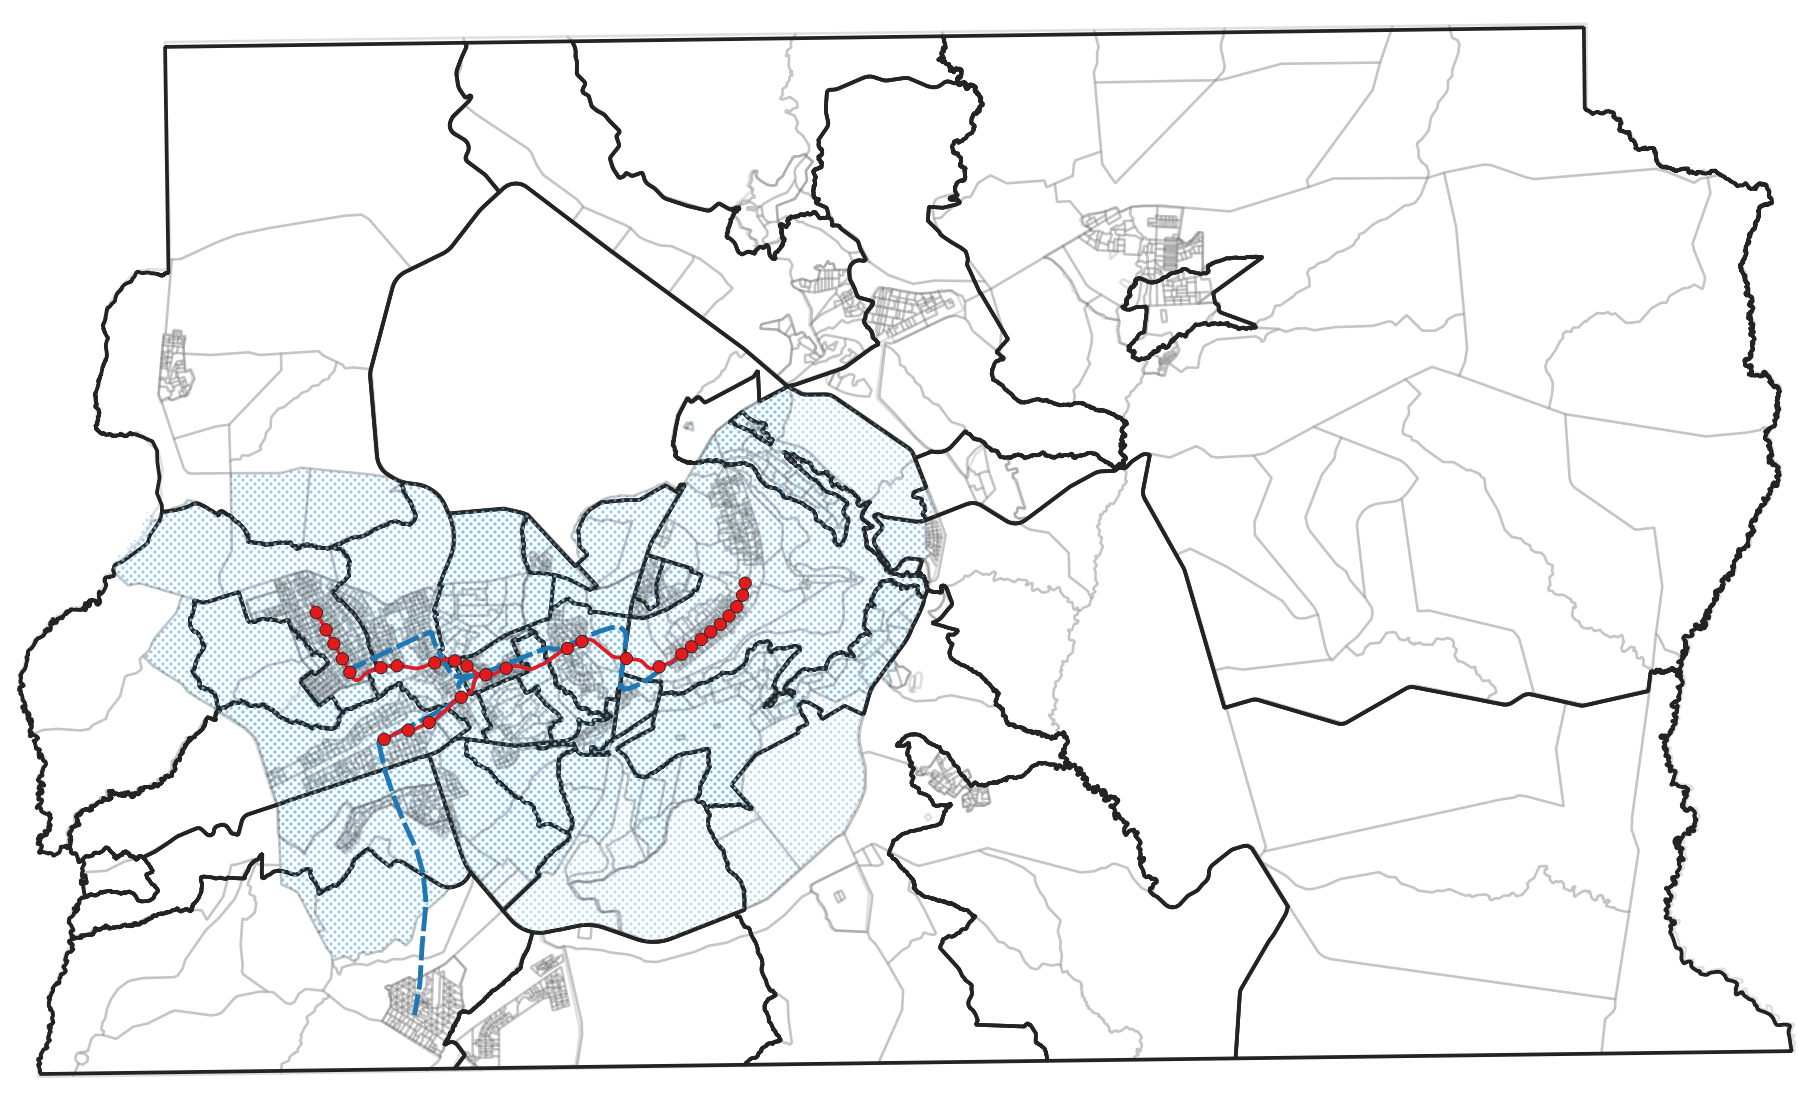
\includegraphics[width=\textwidth]{images/bsb2000.png}
        \caption{\footnotesize Census tracts (2000), subway lines (built and planned) and stations, Administrative Regions, and 10 km buffer.}
    \end{subfigure}
    \hfill
    \begin{subfigure}[b]{0.49\textwidth}
        \centering
        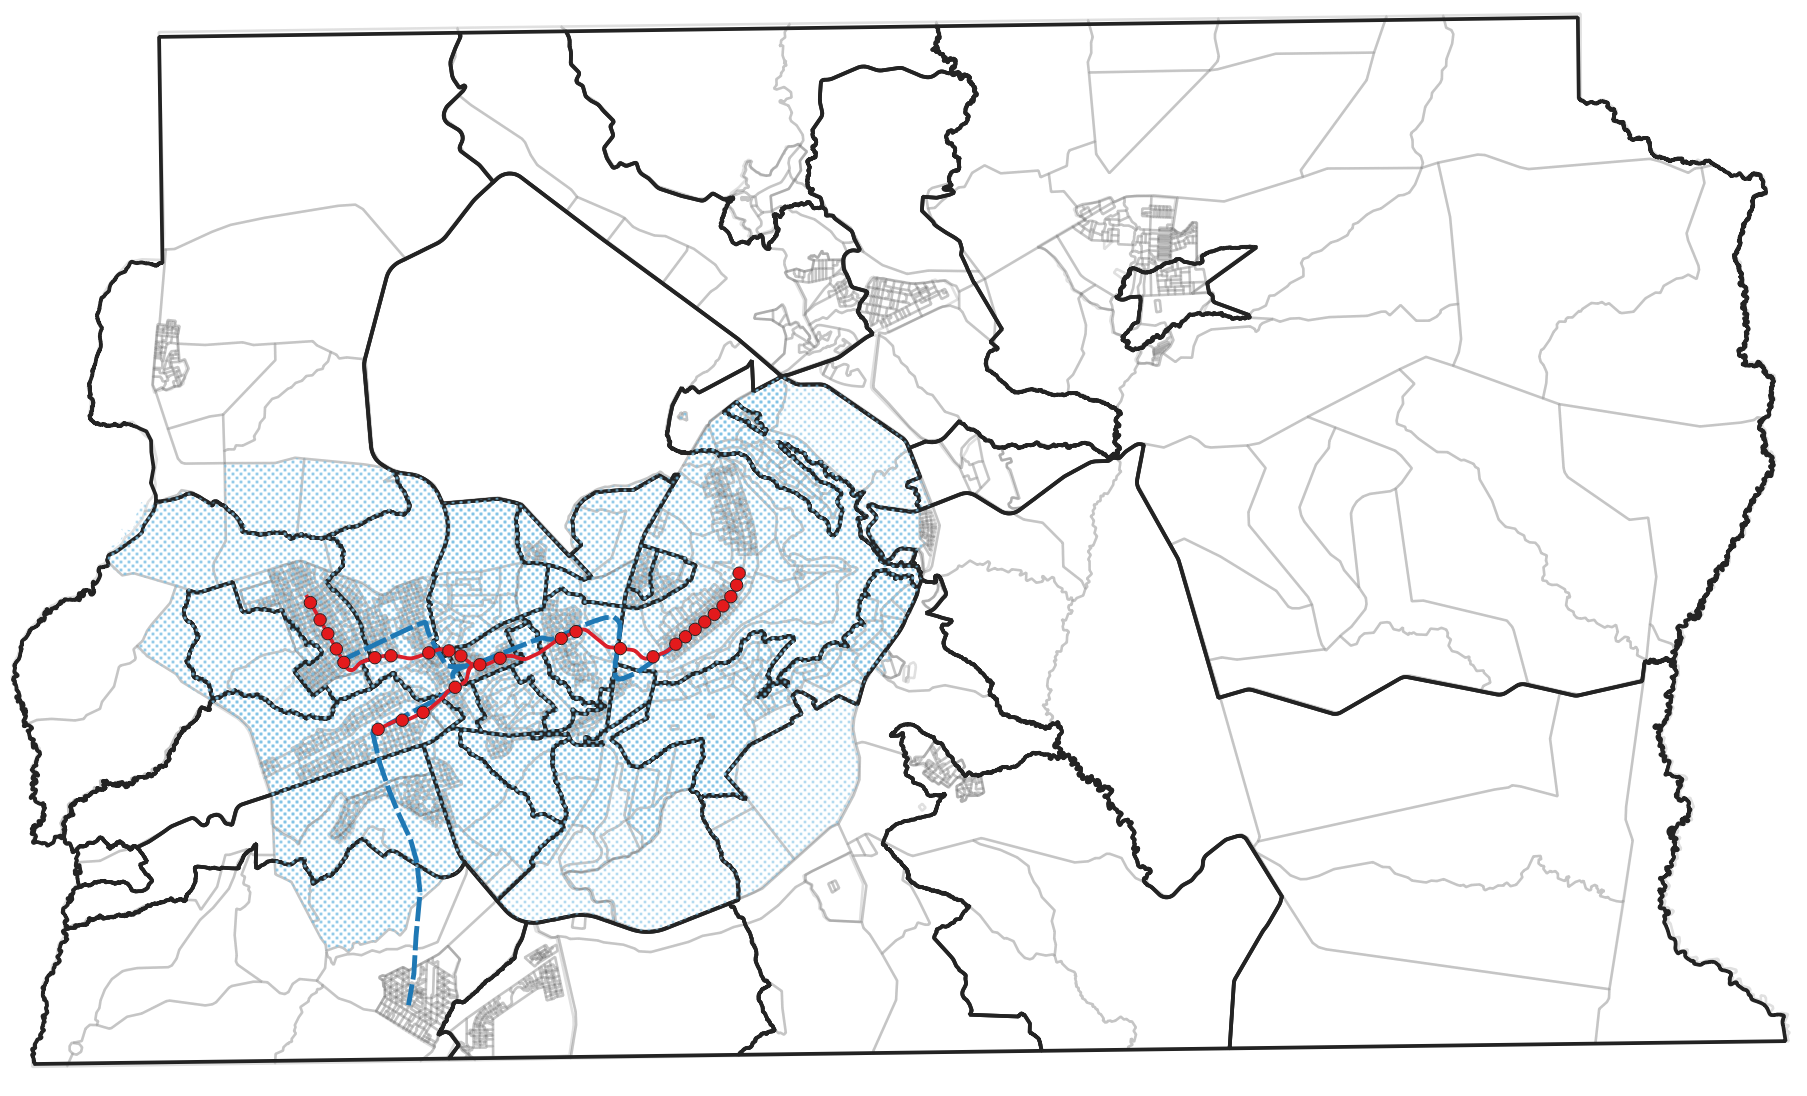
\includegraphics[width=\textwidth]{images/bsb2010.png}
        \caption{\footnotesize Harmonized census tracts (2010), subway lines (built and planned) and stations, Administrative Regions, and 10 km buffer.}
    \end{subfigure}
    \label{fig:1}
\end{figure}

Table~\ref{tab:descriptive} reports summary statistics separately for exposed ($\leq 1$ km from the nearest station) and non-exposed ($>1$ km) census tracts in 2000 and 2010.\footnote{Some demographic and educational composition variables were not reported in the 2010 Census extracts used in this study. This is not a concern for our empirical strategy, since these variables enter the regressions only as baseline (2000) controls.} Of the 1,860 tracts within 10 km of the network in 2000, 592 (32\%) are classified as exposed and 1,268 (68\%) as non-exposed. In 2000, exposed tracts had a higher mean per capita income (R\$618 vs.\ R\$470) and a lower illiteracy rate (5.5\% vs.\ 6.9\%), consistent with subway stations being located in relatively established urban areas. Both groups experienced substantial nominal income growth between 2000 and 2010 (exposed: R\$618 to R\$1{,}388; non-exposed: R\$470 to R\$1{,}035), reflecting the broad-based income expansion observed throughout Brazil in this period. The raw difference in growth rates between the two groups is modest, which highlights why a causal identification strategy is necessary: unconditional comparisons confound the effect of subway access with pre-existing differences in tract characteristics and common income trends.

\begin{table}[!h]
\centering
\caption{Descriptive statistics by subway exposure --- census tracts within 10 km (2000 and 2010)}
\label{tab:descriptive}
\resizebox{0.7\textwidth}{!}{%
\begin{tabular}{lcccc}
\toprule
 & \multicolumn{2}{c}{Exposed ($\leq$ 1 km)} & \multicolumn{2}{c}{Non-exposed ($>$ 1 km)} \\
\cmidrule(lr){2-3}\cmidrule(lr){4-5}
 & 2000 & 2010 & 2000 & 2010 \\
Number of tracts & 592 & 618 & 1,268 & 1,269 \\
\midrule
\multicolumn{5}{l}{\textit{Panel A: Outcome}} \\[2pt]
Per capita income (R\$) & 618 & 1{,}388 & 470 & 1{,}035 \\
 & (569) & (1{,}060) & (521) & (1{,}046) \\[4pt]
\midrule
\multicolumn{5}{l}{\textit{Panel B: Geographic controls}} \\[2pt]
Distance to CBD (meters) & 16{,}367 & --- & 17{,}234 & --- \\
 & (7{,}686) &   & (8{,}522) &  \\[4pt]
Distance to nearest road (meters) & 1{,}141 & --- & 941 & --- \\
 & (816) &   & (719) &  \\[4pt]
\midrule
\multicolumn{5}{l}{\textit{Panel C: Socioeconomic baseline (2000)}} \\[2pt]
Population & 706 & 712 & 816 & 1{,}024 \\
 & (289) & (975) & (298) & (1{,}708) \\[4pt]
Share of illiterate residents & 0.055 & --- & 0.069 & --- \\
 & (0.055) &   & (0.050) &  \\[4pt]
Share with college degree & 0.015 & --- & 0.012 & --- \\
 & (0.024) &   & (0.025) &  \\[4pt]
Share aged 65 or older & 0.049 & --- & 0.034 & --- \\
 & (0.036) &   & (0.025) &  \\[4pt]
\bottomrule
\end{tabular}%
}
\scriptsize
\begin{flushleft}
\textit{Note}: Standard deviations in parentheses. Exposed tracts lie within 1 km of the nearest subway station; non-exposed tracts lie between 1 km and 10 km. Geographic and socioeconomic variables enter the regressions as 2000 baseline characteristics. Statistics for 2010 are not reported for variables not available in the 2010 Census extracts. The number of tracts differs between the two census years because 63 of the 1,905 tracts within 10 km appear in only one of the censuses (45 only in 2010, 18 only in 2000); the regressions use tracts observed in both years.
\end{flushleft}
\end{table}
